\begin{frame}{Quadrilateral excercise}
\begin{enumerate}
\conti
\item A farmer was having a field in the form of a
parallelogram PQRS . She took any point A on
RS and joined it to points P and Q. In how
many parts the fields is divided? What are the
shapes of these parts? The farmer wants to sow
wheat and pulses in equal portions of the field
separately. How should she do it?
\seti
\end{enumerate}
\begin{itemize}
\item \textbf{Solution} :
\begin{center}
\documentclass{article}
\usepackage{tikz}
\usetikzlibrary{shapes.geometric,calc,angles,positioning,intersections,quotes,decorations,babel,patterns,fit}
\usepackage{tkz-euclide}
\usetkzobj{all}
\begin{document}
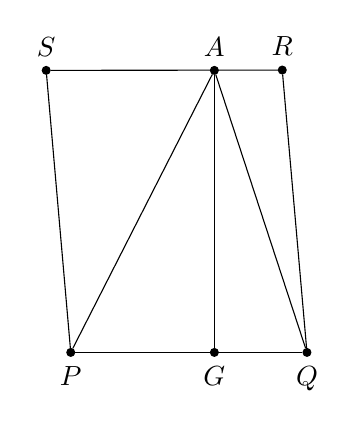
\begin{tikzpicture}
[scale =0.6,>=stealth,point/.style = {draw, circle, fill = black, inner sep = 1pt},]
\node (S) at (-0.52,5.97)[point,label=above :$S$] {};
\node (P) at (0,0)[point,label=below :$P$] {};
\node (A) at (3.04,5.97)[point,label=above :$A$] {};
\node (R) at (4.477,5.977)[point,label=above :$R$] {};
\node (G) at (3.04,0)[point,label=below:$G$] {};
\node (Q) at (5,0)[point,label=below :$Q$] {};
\draw (S)--(P);
\draw (P)--(Q);
\draw (Q)--(R);
\draw (R)--(S);
\draw (A)--(P);
\draw (A)--(Q);
\draw (A)--(G);
\end{tikzpicture}
\end{document}
\end{center}
\end{itemize}
\end{frame}
\begin{frame}
\begin{itemize}
\item PQ = 5\\
\item SP = 6\\
\item AG = 6\\
\item$\triangle$ APQ = $\triangle$PAS + $\triangle$ QAR\\ 
\item$\triangle$ APQ = $\frac{1}{2}$ X l X b\\
$\triangle$ APQ = $\frac{1}{2}$ X 6 X 5\\
$\triangle$ APQ = 15$cm^2$
\item$\triangle$ PAS = $\frac{1}{2}$ X l X b\\
$\triangle$ PAS = $\frac{1}{2}$ X 6 X 3\\
$\triangle$ PAS = 9$cm^2$\\
\item$\triangle$ QRA = $\frac{1}{2}$ X l X b\\
$\triangle$ QRA = $\frac{1}{2}$ X 6 X 2\\
$\triangle$ QRA = 6$cm^2$\\
\item 6 + 9 = 15
\item Hence Area of $\triangle$APQ = Area of $\triangle$PAS + Area of $\triangle$QAR\\
\end{itemize}
\end{frame}
\begin{frame}
\begin{itemize}
\item  After joining the point A to p and Q, the feild is divided into 3 parts.\\
\item All the three parts are in triangle shape.\\
As PQRS is a parallelogram so\\
\end{itemize}
\begin{align*}
\textit{Area of PQRS} = \textit{Area of} \triangle{APS} + \triangle{ARQ} + \triangle{PAQ} --(1)\\
\textit{Area of triangle is half of parallelogram}\\\textit{if they have same base and lie between same parallel lines}. \\
\textit{Area of} \triangle{PAQ} = \frac{1}{2} \textit{Area of PQRS}\\
\triangle{PAQ} = \frac{1}{2}\textit{area}(\triangle{APS} + \triangle{ARQ} + \triangle{APQ}\\
2\triangle{PAQ} - \triangle{PAQ} = \textit{area(}\triangle{APS} + \triangle{ARQ}\textit{)}\\
\triangle{PAQ} = \triangle{APS} + \triangle{ARQ}\\
\textit{Hence the farmer can sow wheat in} \triangle{PAQ} \textit{and pulses in} \triangle{APS} and \triangle{ARQ}\\
\end{align*}
\end{frame}
\begin{frame}
\begin{figure}
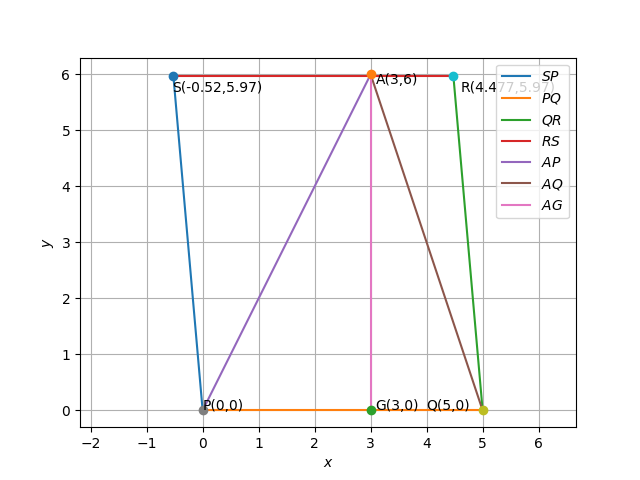
\includegraphics[scale=.5]{./CODES/quad/NEWQUAD.png}\\
\begin{itemize}
\item \url{https://github.com/pratibha444/GEOMETRY/blob/master/figs/FARM.tex}\\
\item \url{https://github.com/pratibha444/GEOMETRY/blob/master/CODES/quad/QUAD_EXCERCISE.py}
\end{itemize}
\seti
\end{figure}
\end{frame}
